\section{Statistical Approaches}


\begin{frame}
  \frametitle{Statistical Approaches}
  Assume that the objects in a data set are \textbf{\color{airforceblue}generated by a stochastic process} (a generative model).
  \begin{itemize}
  \item \textbf{Idea:}
    \begin{itemize}
    \item Learn a generative model fitting the given data set, and then identify the objects in low-probability regions of the model as outliers.
    \end{itemize}
  \item \textbf{Methods divided into two categories:}
    \begin{itemize}
    \item Parametric vs. non-parametric.
    \end{itemize}
  \item \textbf{Parametric method}
    \begin{itemize}
    \item Assumes that the normal data is generated \\
      by a parametric distribution with parameter $\theta$.
    \item The probability density function of the parametric distribution $f(x, \theta)$ \\
      gives the probability that object $x$ is generated by the distribution.
    \item The smaller this value, the more likely $x$ is an outlier.
    \end{itemize}
  \end{itemize}
\end{frame}


\begin{frame}
  \frametitle{Statistical Approaches (2)}
  \begin{itemize}
  \item \textbf{Non-parametric method:}
    \begin{itemize}
    \item Do not assume an a-priori statistical model \\
      and determine the model from the input data.
    \item Not completely parameter-free, \\
      but consider number and nature of the parameters to be flexible and \\ not fixed in advance.
    \item \textbf{Examples:} \textbf{\color{airforceblue}histogram} and kernel-density estimation.
    \end{itemize}
  \end{itemize}
\end{frame}


\begin{frame}
  \frametitle{Parametric Methods I: \\ Detection of Univariate Outliers Based on Normal Distribution}
  \begin{itemize}
  \item Univariate data:
    \begin{itemize}
    \item A data set involving only one attribute or variable.
    \end{itemize}
  \item Assumption:
    \begin{itemize}
    \item Data are generated from a normal distribution.
    \end{itemize}
  \item Learn the parameters from the input data, and identify the points with low probability as outliers.
    \begin{itemize}
    \item Use the \textbf{\color{airforceblue}maximum-likelihood method} to estimate $\mu$ and $\sigma$.
    \end{itemize}
  \end{itemize}
\end{frame}


\begin{frame}
  \frametitle{The Maximum Likelihood Estimate of $\mu$}
  \begin{itemize}
  \item \textbf{Assumption:}
    \begin{itemize}
    \item Data is generated by an underlying Gaussian process. \\
      Thus, the likelihood function $\mathcal{L}$ is the Gaussian process itself:
      \begin{align}
        \mathcal{L}(\mathbf{X}) = \text{P}(\mathbf{X} \; \vert \; \theta) = \mathcal{N}(\mathbf{X} \; \vert \; \theta) = \mathcal{N}(\mathbf{X} \; \vert \; \mu, \sigma).
      \end{align}
    \end{itemize}
  \item We need to find good estimates for $\mu$ and $\sigma$:
    \begin{align}
      \mu_{\text{MLE}} = \text{argmax}_{\mu} \; \mathcal{N}(\mathbf{X} \; \vert \; \mu, \sigma),\\
      \sigma_{\text{MLE}} = \text{argmax}_{\sigma} \; \mathcal{N}(\mathbf{X} \; \vert \; \mu, \sigma).
    \end{align}
  \item To make computation easier, as the product of probabilities $\prod$ turns into sums $\sum$ under the $\log$-function, we apply the logarithm. As $\log$ is monotonically increasing it holds that $\text{argmax}_{\theta} \; \log f(\theta) = \text{argmax}_{\theta} \; f(\theta)$.
  \end{itemize}
\end{frame}


\begin{frame}
  \frametitle{The Maximum Likelihood Estimate of $\mu$}
  \begin{itemize}
  \item We seek for the best parameters $\theta = \{\mu, \sigma\}$ for some dataset $\mathbf{X} = \{\mathbf{x}_1,\ldots,\mathbf{x}_n\}$ of $n$ data points. Thus we take the sum of the respective logarithms applied to the Gaussian:
    \begin{align}
      \log\left(\mathcal{N}(\mathbf{X} \; \vert \; \theta)\right) = \sum_{i=1}^{n} \log\left( \mathcal{N}(\mathbf{x}_i \; \vert \; \theta)\right) = \sum_{i=1}^{n} \log\left( \mathcal{N}(\mathbf{x}_i \; \vert \; \mu, \sigma)\right).
    \end{align}
  \item The log-likelihood function then reads as:
    \begin{align}
      \sum_{i=1}^{n} \log\left(\mathcal{N}(\mathbf{x}_i \; \vert \; \mu, \sigma)\right) = \sum_{i=1}^{n} \log\left(\frac{1}{\sqrt{2\pi\sigma^2}} \cdot \exp \left( -\frac{1}{2} \left( \frac{(\mathbf{x_i}-\mu)^2}{\sigma^2} \right) \right)\right).
    \end{align}
  \item Note, that we took a simplification here. The full covariance matrix $\Sigma$ is replaced keeping only the diagonal elements $\sigma^2$, which is the variance. This is known as the assumption of diagonal covariance matrices.
  \end{itemize}
\end{frame}


\begin{frame}
  \frametitle{The Maximum Likelihood Estimate of $\mu$}
  \begin{itemize}
  \item Next, we use some algebra to get the log-likelihood, denoted by $\log \mathcal{L}(\mathbf{X})$, into a nicer form:
    \begin{align}
      \log\left(\mathcal{L}(\mathbf{X})\right) &= \sum_{i=1}^{n} \log\left(\frac{1}{\sqrt{2\pi\sigma^2}} \cdot \exp\left( -\frac{1}{2} \left( \frac{(\mathbf{x}_i-\mu)^2}{\sigma^2} \right)\right)\right) \\
                                               &= \sum_{i=1}^{n} \log\left(\frac{1}{\sqrt{2\pi\sigma^2}}\right) + \log\left(\exp\left( -\frac{1}{2} \left( \frac{(\mathbf{x}_i-\mu)^2}{\sigma^2} \right)\right)\right)\\
                                               &= \sum_{i=1}^{n} \log(1) - \log(\sqrt{2\pi\sigma^2}) + \log\left(\exp\left( -\frac{1}{2} \left( \frac{(\mathbf{x}_i-\mu)^2}{\sigma^2} \right)\right)\right)\\
                                               &= \sum_{i=1}^{n} \log(1) - \log\left(\sqrt{2\pi\sigma^2}\right) - \frac{1}{2} \left( \frac{(\mathbf{x}_i-\mu)^2}{\sigma^2} \right) \cdot \log(e).
    \end{align}
  \item We simplify the computation taking $\log$ with base $e$. Thus $\log_e e = 1$. \\
    It also applies, regardless of base, that $\log(1) = 0$.
  \end{itemize}
\end{frame}


\begin{frame}
  \frametitle{The Maximum Likelihood Estimate of $\mu$}
  \begin{itemize}
  \item Applying the logarithm with base $e$ yields:
    \begin{align}
      \log\left(\mathcal{L}(\mathbf{X})\right) &= \sum_{i=1}^{n} - \log\left(\sqrt{2\pi\sigma^2}\right) -\frac{1}{2} \left( \frac{(\mathbf{x}_i-\mu)^2}{\sigma^2} \right)\\
                                               &= \sum_{i=1}^{n} - \frac{1}{2} \log\left(2\pi\sigma^2\right) -\frac{1}{2} \left( \frac{(\mathbf{x}_i-\mu)^2}{\sigma^2} \right) \\
                                               &= - \frac{n}{2} \log\left(2\pi\sigma^2\right) + \sum_{i=1}^{n} -\frac{1}{2} \left( \frac{(\mathbf{x}_i-\mu)^2}{\sigma^2} \right)\\
                                               &= - \frac{n}{2} \log\left(2\pi\sigma^2\right) - \frac{1}{2\sigma^2} \sum_{i=1}^{n} (\mathbf{x}_i-\mu)^2.
    \end{align}
  \end{itemize}
\end{frame}


\begin{frame}
  \frametitle{The Maximum Likelihood Estimate of $\mu$}
  \begin{itemize}
  \item In order to get $\text{argmax}_\mu \log\left(\mathcal{L}(\mathbf{X})\right)$ we have to do two things:
    \begin{itemize}
    \item[1.] Derive the partial derivative of the function with respect to the parameter.
    \item[2.] Set the partial derivative to zero, and solve for $\mu$.
    \end{itemize}
  \item In the same way we get $\text{argmax}_\sigma \; \log\left(\mathcal{L}(\mathbf{X})\right)$. Thus,
    \begin{align}
      \text{argmax}_\mu \; \log\left(\mathcal{L}(\mathbf{X})\right) := \frac{\partial \log\left(\mathcal{L}(\mathbf{X})\right)}{\partial \mu} = 0.
    \end{align}
  \item We need to find the following partial derivative:
    \begin{align}
      \frac{\partial \log\left(\mathcal{L}(\mathbf{X})\right)}{\partial \mu} = \frac{\partial}{\partial\mu} \left( - \frac{n}{2} \log\left(2\pi\sigma^2\right) -\frac{1}{2\sigma^2} \sum_{i=1}^{n} (\mathbf{x}_i-\mu)^2 \right).
    \end{align}
  \end{itemize}
\end{frame}


\begin{frame}
  \frametitle{The Maximum Likelihood Estimate of $\mu$}
  \begin{itemize}
  \item We start to simplify our partial derivative:
    \begin{align}
      \frac{\partial \log\left(\mathcal{L}(\mathbf{X})\right)}{\partial \mu} &= \frac{\partial}{\partial\mu} \left( - \frac{n}{2} \log\left(2\pi\sigma^2\right) -\frac{1}{2\sigma^2} \sum_{i=1}^{n} (\mathbf{x}_i-\mu)^2 \right)\\
                                                                             &= \frac{\partial}{\partial\mu} \left( - \frac{n}{2} \log\left(2\pi\sigma^2\right)\right) + \frac{\partial}{\partial\mu}\left(-\frac{1}{2\sigma^2} \sum_{i=1}^{n} (\mathbf{x}_i-\mu)^2 \right)\\
                                                                             &= 0 + \frac{\partial}{\partial\mu}\left(-\frac{1}{2\sigma^2} \sum_{i=1}^{n} (\mathbf{x}_i-\mu)^2 \right)\\
                                                                             &= \frac{\partial}{\partial\mu}\left(-\frac{1}{2\sigma^2} \sum_{i=1}^{n} (\mathbf{x}_i-\mu)^2 \right).
    \end{align}
  \end{itemize}
\end{frame}


\begin{frame}
  \frametitle{The Maximum Likelihood Estimate of $\mu$}
  \begin{itemize}
  \item Next, we move the partial operator inside the sum:
    \begin{align}
      \frac{\partial \log\left(\mathcal{L}(\mathbf{X})\right)}{\partial \mu} &= \frac{\partial}{\partial\mu}\left(-\frac{1}{2\sigma^2} \sum_{i=1}^{n} (\mathbf{x}_i-\mu)^2 \right) \\
                                                                             &= \frac{\partial}{\partial\mu}\left(\sum_{i=1}^{n}-\frac{1}{2\sigma^2} (\mathbf{x}_i-\mu)^2 \right)\\
                                                                             &= \sum_{i=1}^{n} \frac{\partial}{\partial\mu}\left(-\frac{1}{2\sigma^2} (\mathbf{x}_i-\mu)^2\right)\\
                                                                             &= \sum_{i=1}^{n} \left(\frac{\partial}{\partial\mu}\left(-\frac{1}{2\sigma^2}\right) \cdot (\mathbf{x}_i - \mu)^2 + \left( - \frac{1}{2\sigma^2} \right) \cdot \frac{\partial}{\partial\mu} (\mathbf{x}_i-\mu)^2\right).
    \end{align}
  \end{itemize}
\end{frame}


\begin{frame}
  \frametitle{The Maximum Likelihood Estimate of $\mu$}
  \begin{itemize}
  \item After having applied the product rule, some of the terms drop out:
    \begin{align}
      \frac{\partial \log\left(\mathcal{L}(\mathbf{X})\right)}{\partial \mu} &= \sum_{i=1}^{n} \left(\frac{\partial}{\partial\mu}\left(-\frac{1}{2\sigma^2}\right) \cdot (\mathbf{x}_i - \mu)^2 + \left( - \frac{1}{2\sigma^2} \right) \cdot \frac{\partial}{\partial\mu} (\mathbf{x}_i-\mu)^2\right) \\
                                                                             &= \sum_{i=1}^{n} \left(0 + \left( - \frac{1}{2\sigma^2} \right) \cdot \frac{\partial}{\partial\mu} (\mathbf{x}_i-\mu)^2\right)\\
                                                                             &= - \frac{1}{2\sigma^2} \sum_{i=1}^{n} \frac{\partial}{\partial\mu} (\mathbf{x}_i-\mu)^2.
    \end{align}
  \item Using the chain rule we yield:
    \begin{align}
      \frac{\partial \log\left(\mathcal{L}(\mathbf{X})\right)}{\partial \mu} &= - \frac{1}{2\sigma^2} \sum_{i=1}^{n}  2(\mathbf{x}_i-\mu) \cdot -1 = \frac{1}{\sigma^2} \sum_{i=1}^{n}  (\mathbf{x}_i-\mu).
    \end{align}
  \end{itemize}
\end{frame}


\begin{frame}
  \frametitle{The Maximum Likelihood Estimate of $\mu$}
  \begin{columns}
    \begin{column}{0.5\textwidth}
      \begin{itemize}
      \item Finally, we set this equation to $0$ and solve the fixpoint equation according to $\mu$:
        \begin{align}
          \frac{1}{\sigma^2} \sum_{i=1}^{n} (\mathbf{x}_i-\mu) &= 0, \\
          \sum_{i=1}^{n} (\mathbf{x}_i-\mu) &= 0, \\
          \sum_{i=1}^{n} \mathbf{x}_i- \sum_{i=1}^{n} \mu &= 0,
        \end{align}
      \end{itemize}
    \end{column}
    \begin{column}{0.5\textwidth}
      \centering
      \begin{align}
        0 &= \sum_{i=1}^{n} \mathbf{x}_i- n \mu , \\
        n \mu &= \sum_{i=1}^{n} \mathbf{x}_i,\\
        \mu &= \frac{1}{n} \sum_{i=1}^{n}\mathbf{x}_i.
      \end{align}
    \end{column}
  \end{columns}
\end{frame}


\begin{frame}
  \frametitle{The Maximum Likelihood Estimate of $\sigma$}
  \begin{itemize}
  \item We proceed similar for $\sigma$, and solve the partial differential equation according to our second parameter. But, first we simplify again the equation to something more handy:
    \begin{align}
      \frac{\partial \log\left(\mathcal{L}(\mathbf{X})\right)}{\partial \sigma^2} &= \frac{\partial}{\partial\sigma^2} \left(-\frac{n}{2} \log\left(2\pi\sigma^2\right) - \frac{1}{2\sigma^2} \sum_{i=1}^{n} (\mathbf{x}_i-\mu)^2 \right)\\
                                                                                  &= \frac{\partial}{\partial\sigma^2} \left(-\frac{n}{2} \log\left(2\pi\sigma^2\right)\right) + \frac{\partial}{\partial\sigma^2}\left(-\frac{1}{2\sigma^2} \sum_{i=1}^{n} (\mathbf{x}_i-\mu)^2 \right).
    \end{align}
  \item We apply the product rule to the log-likelihood function:
    \begin{align*}
      \frac{\partial \log\left(\mathcal{L}(\mathbf{X})\right)}{\partial \sigma^2} &= \frac{\partial}{\partial\sigma^2}(-\frac{n}{2}) \cdot \log\left(2\pi\sigma^2\right) - \frac{n}{2} \cdot \frac{\partial}{\partial\sigma^2} \log\left(2\pi\sigma^2\right) + \frac{\partial}{\partial\sigma^2}\left( -\frac{1}{2\sigma^2} \sum_{i=1}^{n} (\mathbf{x}_i-\mu)^2 \right).
    \end{align*}
  \end{itemize}
\end{frame}



\begin{frame}
  \frametitle{The Maximum Likelihood Estimate of $\sigma$}
  \begin{itemize}
  \item Again some of the terms drop out:
    \begin{align}
      \frac{\partial \log\left(\mathcal{L}(\mathbf{X})\right)}{\partial \sigma^2} &= - \frac{n}{2} \cdot \frac{\partial}{\partial\sigma^2} \log\left(2\pi\sigma^2\right) + \frac{\partial}{\partial\sigma^2}\left( -\frac{1}{2\sigma^2} \sum_{i=1}^{n} (\mathbf{x}_i-\mu)^2 \right).
    \end{align}
  \item Using the chain rule we yield:
    \begin{align}
      \frac{\partial \log\left(\mathcal{L}(\mathbf{X})\right)}{\partial \sigma^2} &= - \frac{n}{2} \cdot \frac{1}{2\pi\sigma^2} 2\pi + \frac{\partial}{\partial\sigma^2}\left( -\frac{1}{2\sigma^2} \sum_{i=1}^{n} (\mathbf{x}_i-\mu)^2 \right),\\
                                                                                  &= - \frac{n}{2\sigma^2} + \frac{\partial}{\partial\sigma^2}\left( -\frac{1}{2\sigma^2} \sum_{i=1}^{n} (\mathbf{x}_i-\mu)^2 \right).
    \end{align}
  \end{itemize}
\end{frame}


\begin{frame}
  \frametitle{The Maximum Likelihood Estimate of $\sigma$}
  \begin{itemize}
  \item Moving the partial operator inside the sum and applying the product rule yields:
    \begin{align}
      \frac{\partial \log\left(\mathcal{L}(\mathbf{X})\right)}{\partial \sigma^2} &= -\frac{n}{2\sigma^2} + \sum_{i=1}^{n} \frac{\partial}{\partial\sigma^2}\left(-\frac{1}{2\sigma^2} (\mathbf{x}_i-\mu)^2 \right). \\
                                                                                  &= -\frac{n}{2\sigma^2} + \sum_{i=1}^{n} \left(\frac{\partial}{\partial\sigma^2} \left(-\frac{1}{2\sigma^2}\right) (\mathbf{x}_i-\mu)^2 - \frac{1}{2\sigma^2} \cdot \frac{\partial}{\partial\sigma^2} (\mathbf{x}_i-\mu)^2 \right). \\
                                                                                  &= -\frac{n}{2\sigma^2} + \sum_{i=1}^{n} \left(\frac{\partial}{\partial\sigma^2} \left(-\frac{1}{2\sigma^2}\right) (\mathbf{x}_i-\mu)^2\right).
    \end{align}
  \item We switch the notation a little, such that the next steps become more intuitive:
    \begin{align}
      \frac{\partial \log\left(\mathcal{L}(\mathbf{X})\right)}{\partial \sigma^2} &= -\frac{n}{2\sigma^2} + \sum_{i=1}^{n} \left(\frac{\partial}{\partial\sigma^2} \left(-\frac{1}{2}\cdot \sigma^{-2}\right) (\mathbf{x}_i-\mu)^2\right).
    \end{align}
  \end{itemize}
\end{frame}


\begin{frame}
  \frametitle{The Maximum Likelihood Estimate of $\sigma$}
  \begin{itemize}
  \item Once again we use the chain rule to simplify our log-likelihood derivative:
    \begin{align}
      \frac{\partial \log\left(\mathcal{L}(\mathbf{X})\right)}{\partial \sigma^2} &= -\frac{n}{2\sigma^2} + \sum_{i=1}^{n} \left(\frac{\partial}{\partial\sigma^2} \left(-\frac{1}{2} \right) \cdot \sigma^{-2} - \frac{1}{2} \frac{\partial}{\partial\sigma^2} \sigma^{-2} \cdot (\mathbf{x}_i-\mu)^2\right) \\
                                                                                  &=  -\frac{n}{2\sigma^2} + \sum_{i=1}^{n} - \frac{1}{2} \frac{\partial}{\partial\sigma^2} \sigma^{-2} \cdot (\mathbf{x}_i-\mu)^2 \\
                                                                                  &=  -\frac{n}{2\sigma^2} + \sum_{i=1}^{n} - \frac{1}{2} \frac{\partial}{\partial\sigma^2} (\sigma^{2})^{-1} \cdot (\mathbf{x}_i-\mu)^2 \\
                                                                                  &=  -\frac{n}{2\sigma^2} + \sum_{i=1}^{n} - \frac{1}{2} \cdot -1 \cdot (\sigma^{2})^{-2} \cdot 1 \cdot (\mathbf{x}_i-\mu)^2\\
                                                                                  &=  -\frac{n}{2\sigma^2} + \sum_{i=1}^{n} \frac{1}{2\sigma^4} (\mathbf{x}_i-\mu)^2.
    \end{align}
  \end{itemize}
\end{frame}


\begin{frame}
  \frametitle{The Maximum Likelihood Estimate of $\sigma$}
  \begin{itemize}
  \item We can simplify the equation a little more:
    \begin{align}
      \frac{\partial \log\left(\mathcal{L}(\mathbf{X})\right)}{\partial \sigma^2} &= -\frac{n}{2\sigma^2} + \frac{1}{2\sigma^4} \sum_{i=1}^{n} (\mathbf{x}_i-\mu)^2 = -\frac{1}{2\sigma^2} \left( -n + \frac{1}{\sigma^2} \sum_{i=1}^{n} (\mathbf{x}_i-\mu)^2\right).
    \end{align}
  \item Finally, we set the equation to $0$ and solve the fixpoint equation:
    \begin{align}
      -\frac{1}{2\sigma^2} \left( -n + \frac{1}{\sigma^2} \sum_{i=1}^{n} (\mathbf{x}_i-\mu)^2\right) &= 0, \\
      -n + \frac{1}{\sigma^2} \sum_{i=1}^{n} (\mathbf{x}_i-\mu)^2 &= 0, \\
      \frac{1}{n} \sum_{i=1}^{n} (\mathbf{x}_i-\mu)^2 &= \sigma^2.
    \end{align}
  \end{itemize}
\end{frame}


\begin{frame}
  \frametitle{Parametric Methods I: \\ Detection of Univariate Outliers Based on Normal Distribution (2)}
  \begin{itemize}
  \item \textbf{Example:}
    \begin{itemize}
    \item Average temperature: $\{24.0, 28.9, 28.9, 29.0, 29.1, 29.1, 29.2, 29.2, 29.3, 29.4\}$.
    \item For these data with $n = 10$, we have
      \begin{align}
        \widehat{\mu}=28.61, \quad \widehat{\sigma}=\sqrt{2.29}=1.51.
      \end{align}
    \item Then the most deviating value $24.0$ is $4.61$ away form the estimated mean.
    \item $\mu \pm 3\sigma $ contains $99.7\%$ of the data under the assumption of normal distribution.
    \item Because $\frac{4.61}{1.51}  =  3.04  >  3$, \\
      the probability that $24.0$ is generated by a normal distribution is less than $0.15\%$.
      \begin{itemize}
      \item Each \emph{tail} to the left and to the right of the $99.7\%$ has $0.15\%$.
      \end{itemize}
    \item Hence, $24.0$ identified as an outlier.
    \end{itemize}
  \end{itemize}
\end{frame}


\begin{frame}
  \frametitle{Parametric Methods I: The Grubb's Test}
  \begin{itemize}
  \item Univariate outlier detection: The Grubb's test (maximum normed residual test).
    \begin{itemize}
    \item Another statistical method under normal distribution
    \item For each object $x$ in a data set, compute its $z$-score:  $z = \frac{\vert x - \overline{x}\vert}{s}$,
      \begin{itemize}
      \item where $\overline{x}$ is the mean and $s$ the standard deviation of the input data.
      \end{itemize}
    \item $x$ is an outlier, if
      \begin{align}
        z \geq \frac{N-1}{\sqrt{N}} \sqrt{\frac{t^2_{\frac{\alpha}{2N},N-2}}{N-2 + t^2_{\frac{\alpha}{2N},N-2}}},
      \end{align}
    \end{itemize}
    \begin{itemize}
    \item where $t^2_{\frac{\alpha}{2N},N-2}$ is the value taken by a $t$-distribution \\
      at a significance level of $\frac{\alpha}{2N}$, and $N$ is the number of objects in the data set.
    \end{itemize}
  \end{itemize}
\end{frame}


\begin{frame}
  \frametitle{Parametric Methods II: Detection of Multivariate Outliers}
  \begin{itemize}
  \item \textbf{Multivariate data}:
    \begin{itemize}
    \item A data set involving \textbf{\color{airforceblue}two or more attributes} or variables.
    \end{itemize}
  \item \textbf{Transform the multivariate outlier-detection task into a univariate outlier-detection problem.}
  \item \textbf{Method 1: Compute Mahalanobis distance.}
    \begin{itemize}
    \item Let $\mathbf{\overline{o}}$ be the mean vector for a multivariate data set. Mahalanobis distance for an object $\mathbf{o}$ to $\mathbf{\overline{o}}$ is $\Delta(\mathbf{o}, \mathbf{\overline{o}}) = (\mathbf{o} - \mathbf{\overline{o}})^T \mathbf{S}^{-1} (\mathbf{o} - \mathbf{\overline{o}})$ where $\mathbf{S}$ is the covariance matrix.
    \item Use the Grubb's test on this measure to detect outliers.
    \end{itemize}
  \item \textbf{Method 2: Use $\chi^2$ statistic.}
    \begin{itemize}
    \item \vspace{-0.5cm}
      \begin{align}
        \chi^2 = \sum^n_{i=1} \frac{(\mathbf{o}_i-E_i)^2}{E_i},
      \end{align}
    \item where $E_i$ is the mean of the $i$-dimension among all objects, and $n$ is the dimensionality.
    \item If $\chi^2$ statistic is large, then object $\mathbf{o}_i$ is an outlier.
    \end{itemize}
  \end{itemize}
\end{frame}


\begin{frame}
  \frametitle{Parametric Methods III: Using Mixture of Parametric Distributions}
  \begin{itemize}
  \item \textbf{Assuming that data are generated by a normal distribution \\ could sometimes be overly simplified.}
  \item \textbf{Example (right figure):}
    \begin{itemize}
    \item The objects between the two clusters cannot be captured \\
      as outliers since they are close to the estimated mean.
    \end{itemize}
  \item \textbf{Assume the normal data is generated by {\color{airforceblue}two normal distributions.}}
    \begin{itemize}
    \item For any object $\mathbf{o}$ in the data set, the probability that $\mathbf{o}$ is generated by the mixture of the two distributions is given by
      \begin{align}
        \text{P}(\mathbf{o} \; \vert \; \theta_1, \theta_2) = f(\mathbf{o} \; \vert \; \theta_1) + f(\mathbf{o} \; \vert \; \theta_2),
      \end{align}
      where $f_{\theta 1}$ and $f_{\theta 2}$ are the probability density functions of $\theta_1$ and $\theta_2$.
    \item Then use expectation-maximization (EM) algorithm \\
      to learn the parameters $\mu_1, \sigma_1, \mu_2, \sigma_2$ from the data.
    \item An object $\mathbf{o}$ is an outlier if it does not belong to any cluster.
    \end{itemize}
  \end{itemize}
\end{frame}


\begin{frame}
  \frametitle{Non-Parametric Methods:Detection Using Histogram}
  \begin{itemize}
  \item \textbf{The model of normal data is learned from the input data without any apriori structure.}
    \begin{itemize}
    \item Often makes fewer assumptions about the data, and thus can be applicable in more scenarios.
    \end{itemize}
  \item \textbf{Outlier detection using histograms:}
    \begin{itemize}
    \item Figure shows the histogram of purchase amounts in transactions.
    \item A transaction with the amount of $\$7,500$ is an outlier, since only $0.2\%$ \\ of the transactions have an amount higher than $\$5,000$.
    \end{itemize}
  \end{itemize}
  \centering
  \vspace{0.2cm}
  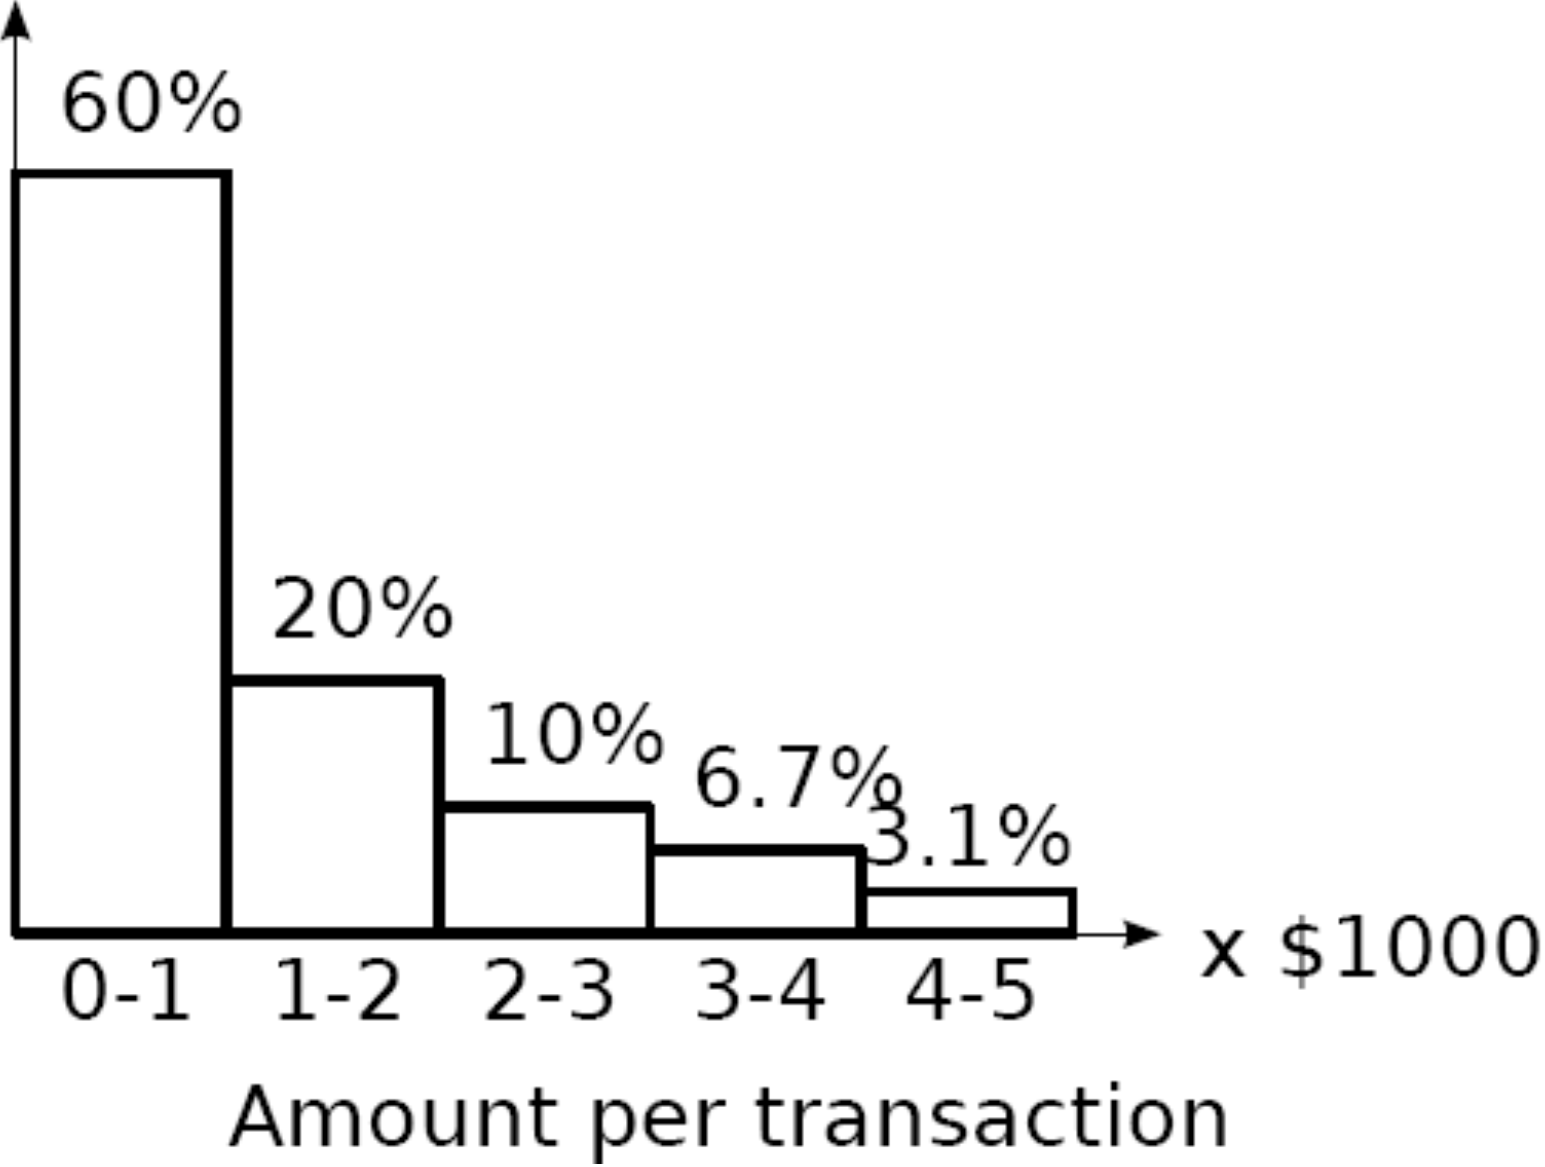
\includegraphics[width=0.25\textwidth]{img/histogram8.png}
\end{frame}


\begin{frame}
  \frametitle{Non-Parametric Methods: Detection Using Histogram (2)}
  \begin{itemize}
  \item \textbf{Problem:}
    \begin{itemize}
    \item Hard to \textbf{\color{airforceblue}choose an appropriate bin size} for histogram.
      \begin{itemize}
      \item Too small bin size $\rightarrow$ normal objects in empty/rare bins, false positive.
      \item Too big bin size $\rightarrow$ outliers in some frequent bins, false negative.
      \end{itemize}
    \end{itemize}
  \item \textbf{Solution:}
    \begin{itemize}
    \item Adopt kernel-density estimation to estimate the probability-density distribution of the data.
      \begin{itemize}
      \item If the estimated density function is high, the object is likely normal.
      \item Otherwise, it is likely an outlier.
      \end{itemize}
    \end{itemize}
  \end{itemize}
\end{frame}
